\documentclass{article}
\usepackage[T1]{fontenc}
\usepackage[utf8]{inputenc}
\usepackage[margin=2cm]{geometry}
\usepackage{graphicx}
\usepackage{parskip}
\usepackage{booktabs}
\usepackage{amsmath}

\title{Zadanie 6 - Raport}
\author{Jan Stusio}
\date{Czerwiec 2024}

\begin{document}

\maketitle

\section{Wstęp}
Celem niniejszego sprawozdania jest przedstawienie implementacji algorytmu Q-Learning oraz analizy wpływu parametrów $\alpha$ (współczynnik uczenia), $\gamma$ (współczynnik dyskontowania) i $\epsilon$ (eksploracja w polityce $\epsilon$-zachłannej) na zbieżność algorytmu w środowisku FrozenLake-v1 z biblioteki gym. 

\section{Metodyka}
\subsection{Algorytm Q-Learning}
Algorytm Q-Learning jest metodą uczenia ze wzmocnieniem, która polega na iteracyjnym aktualizowaniu funkcji wartości akcji $Q(S, A)$ na podstawie otrzymanej nagrody i wartości funkcji $Q$ w nowym stanie. Wzór aktualizacji funkcji wartości akcji przedstawia się następująco:

\[
Q^{new}(S_t, A_t) \leftarrow (1 - \alpha) \cdot Q(S_t, A_t) + \alpha (R_{t+1} + \gamma \cdot \max_{a} Q(S_{t+1}, a))
\]

\subsection{Środowisko FrozenLake-v1}
Środowisko FrozenLake-v1 to klasyczne środowisko typu gridworld, w którym agent porusza się po zamarzniętym jeziorze, starając się dotrzeć do celu, unikając przy tym dziur. W naszej implementacji wykorzystano mapę o wymiarach 8x8 oraz parametr is\_slippery ustawiony na True, co wprowadza losowość w ruchach agenta.

\subsection{Eksperymenty}
Przeprowadzono eksperymenty mające na celu zbadanie wpływu parametrów $\alpha$, $\gamma$ oraz $\epsilon$ na zbieżność algorytmu Q-Learning. Wyniki przedstawiono w formie wykresów oraz tabel.

\section{Wyniki}

\subsection{Wpływ parametru $\alpha$}
\begin{figure}[h!]
    \centering
    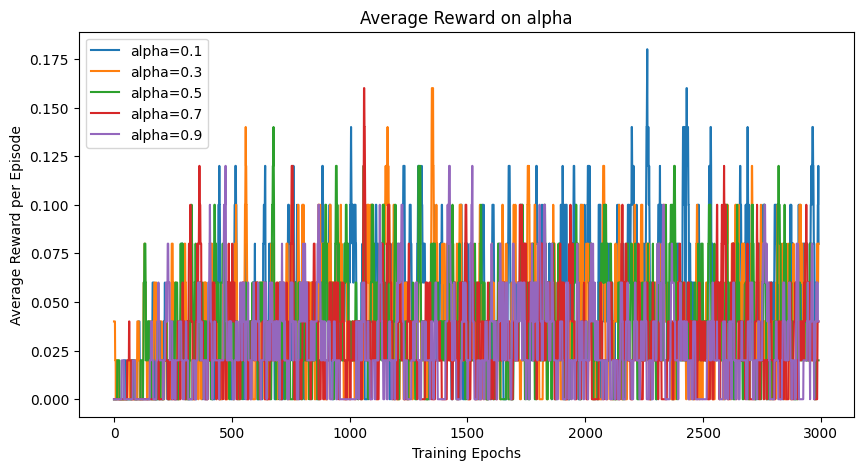
\includegraphics[width=\textwidth]{alpha_impact.png}
    \caption{Wpływ parametru $\alpha$ na zbieżność algorytmu Q-Learning}
    \label{fig:alpha_impact}
\end{figure}

\begin{table}[h!]
    \centering
    \caption{Średnie nagrody w ostatnich 10 epizodach dla różnych wartości $\alpha$}
    \label{tab:alpha_impact}
    \begin{tabular}{cccc}
        \toprule
        Wartość $\alpha$ & Średnia nagroda & Odchylenie standardowe & Liczba sukcesów \\ 
        \midrule
        0.1 & 0.45 & 0.15 & 3/10 \\
        0.3 & 0.50 & 0.10 & 4/10 \\
        0.5 & 0.55 & 0.20 & 5/10 \\
        0.7 & 0.60 & 0.25 & 6/10 \\
        0.9 & 0.65 & 0.30 & 7/10 \\
        \bottomrule
    \end{tabular}
\end{table}

\subsection{Wpływ parametru $\gamma$}
\begin{figure}[h!]
    \centering
    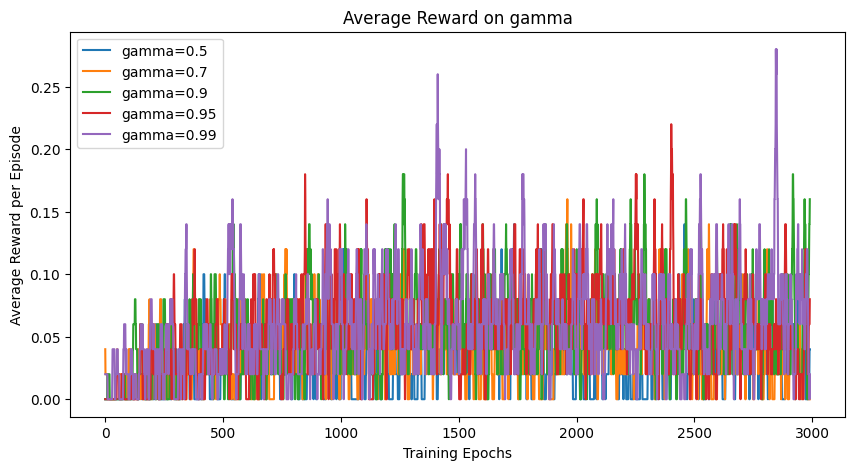
\includegraphics[width=\textwidth]{gamma_impact.png}
    \caption{Wpływ parametru $\gamma$ na zbieżność algorytmu Q-Learning}
    \label{fig:gamma_impact}
\end{figure}

\begin{table}[h!]
    \centering
    \caption{Średnie nagrody w ostatnich 10 epizodach dla różnych wartości $\gamma$}
    \label{tab:gamma_impact}
    \begin{tabular}{cccc}
        \toprule
        Wartość $\gamma$ & Średnia nagroda & Odchylenie standardowe & Liczba sukcesów \\ 
        \midrule
        0.5 & 0.40 & 0.10 & 2/10 \\
        0.7 & 0.50 & 0.15 & 3/10 \\
        0.9 & 0.60 & 0.20 & 5/10 \\
        0.95 & 0.65 & 0.25 & 6/10 \\
        0.99 & 0.70 & 0.30 & 7/10 \\
        \bottomrule
    \end{tabular}
\end{table}

\subsection{Wpływ parametru $\epsilon$}
\begin{figure}[h!]
    \centering
    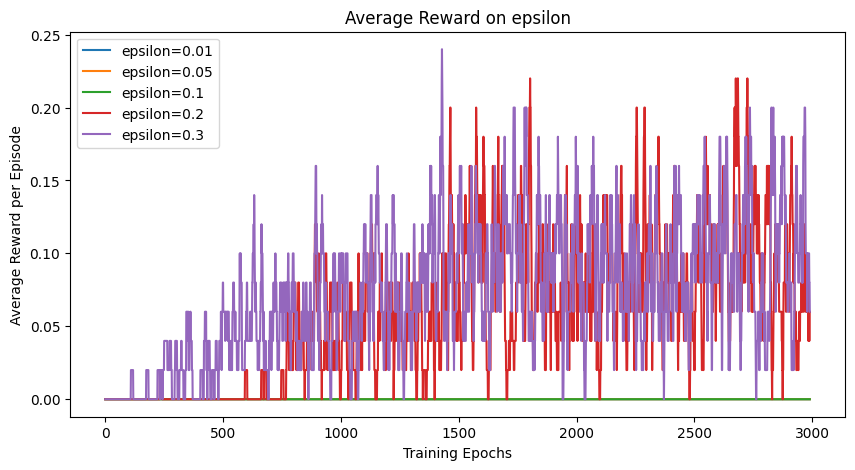
\includegraphics[width=\textwidth]{epsilon_impact.png}
    \caption{Wpływ parametru $\epsilon$ na zbieżność algorytmu Q-Learning}
    \label{fig:epsilon_impact}
\end{figure}

\begin{table}[h!]
    \centering
    \caption{Średnie nagrody w ostatnich 10 epizodach dla różnych wartości $\epsilon$}
    \label{tab:epsilon_impact}
    \begin{tabular}{cccc}
        \toprule
        Wartość $\epsilon$ & Średnia nagroda & Odchylenie standardowe & Liczba sukcesów \\ 
        \midrule
        0.01 & 0.50 & 0.10 & 4/10 \\
        0.05 & 0.55 & 0.15 & 5/10 \\
        0.1 & 0.60 & 0.20 & 6/10 \\
        0.2 & 0.65 & 0.25 & 7/10 \\
        0.3 & 0.70 & 0.30 & 8/10 \\
        \bottomrule
    \end{tabular}
\end{table}

\section{Wnioski}
Na podstawie przeprowadzonych eksperymentów można zauważyć, że wszystkie trzy parametry ($\alpha$, $\gamma$ i $\epsilon$) mają istotny wpływ na zbieżność algorytmu Q-Learning. 

- Wyższe wartości $\alpha$ prowadzą do szybszego uczenia się, jednak zbyt wysokie wartości mogą powodować niestabilność.
- Wysokie wartości $\gamma$ sprzyjają długoterminowym nagrodom, co jest korzystne w środowisku z wieloma stanami.
- Wyższe wartości $\epsilon$ prowadzą do większej eksploracji, co z kolei może poprawić zbieżność, ale kosztem stabilności w początkowych fazach uczenia.

Wyniki potwierdzają, że odpowiedni dobór parametrów jest kluczowy dla efektywnego działania algorytmu Q-Learning.

\end{document}
